\begin{ledgroupsized}[r]{120mm}
\footnotesize 
\pstart 
\noindent\textbf{\"{U}berlieferung:}
\pend
\end{ledgroupsized}
\begin{ledgroupsized}[r]{114mm}
\footnotesize 
\pstart \parindent -6mm
\makebox[6mm][l] {\textit{L}}Konzept: LH XXXV 13, 3 Bl. 35. 1 Bl. 2\textsuperscript{o}. 1 S. auf Bl.~35~v\textsuperscript{o}. Bl. 35~r\textsuperscript{o} leer. Ein Wasserzeichen. \\Cc 2, Nr. 974 \pend
\end{ledgroupsized}
 
\vspace*{5mm}
\begin{ledgroup}
\footnotesize 
\pstart
\noindent\footnotesize{\textbf{Datierungsgr\"{u}nde}: Einen Hinweis auf die Entstehungszeit liefert die Zeichnung [\textit{Fig. 4}]; sie findet sich auch in N.~9, N.~30 und N.~95.
%N. ??
%%= LH35,14,2Bl.114-115 = Excerpta ex Wallisio
%, in N. ??
%%=LH37,05Bl.012 = De detrimento motus. Frottement
%und in N. ??
%=LH35,2,1Bl.273 = Zeichnungen zur Mechanik
Das Wasserzeichen ist durch ein Blatt des von Leibniz eigenhändig datierten Stücks N.~32
%=LH37,05Bl.010-011+006 = De detrimento motus. Pars secunda
für April 1675 belegt.}
\pend
\end{ledgroup}

\vspace*{8mm}
\count\Bfootins=1200
\pstart 
\noindent
\normalsize
[35~v\textsuperscript{o}] Si Motus non nisi situs mutatio esset, (: quod non Cartesium\protect\index{Namensregister}{\textso{Descartes}, Ren\´{e} (1596-1650)} tantum sed et Hugenium\protect\index{Namensregister}{\textso{Huygens}, Christiaan (1629-1695)} sentire video :) duobus corporibus sibi appropinquantibus nihil referret, alterum an \edtext{utrumque, ac si alterutrum, quodnam ex ipsis, moveri dicatur.}{\lemma{utrumque,} \Bfootnote{\textit{(1)}\ moveretur a \textit{(2)}\ ac si [...] dicatur. \textit{L}}} Unde pendulum\protect\index{Sachverzeichnis}{pendulum} \textit{CD} impingat in pendulum \textit{AB}, perinde erit ac si alterum alteri occurreret, \edtext{aequali celeritate unde}{\lemma{occurreret} \Bfootnote{\textit{(1)}\ unde aliamque \textit{(2)}\ aequali celeritate unde \textit{L}\ }} quiesceret utrumque, quod est experientiae\protect\index{Sachverzeichnis}{experientia} adversum. Nam (si nullum adsit Elaterium\protect\index{Sachverzeichnis}{elaterium}) pendulum \textit{AB} a pendulo \textit{CD} nulla motus sui diminutione aufertur. \edtext{Responderi potest huic objectioni pro definitione motus}{\lemma{aufertur.} \Bfootnote{\textit{(1)}\ Sed his responderi potest, etsi motus h \textit{(2)}\ Responderi potest  \textbar\ , \textit{streicht Hrsg.} \textbar\ huic [...] motus \textit{L}\ }} a qua nec ego abhorreo, non de motu hic sed de effectu esse quaestionem, et cum quidlibet fingi possit pro arbitrio, motum generalem exitum quem potest reperire.
\pend
\vspace{3.5em}
\pstart
\hspace{8mm}
\begin{minipage}[c]{0.5\textwidth}
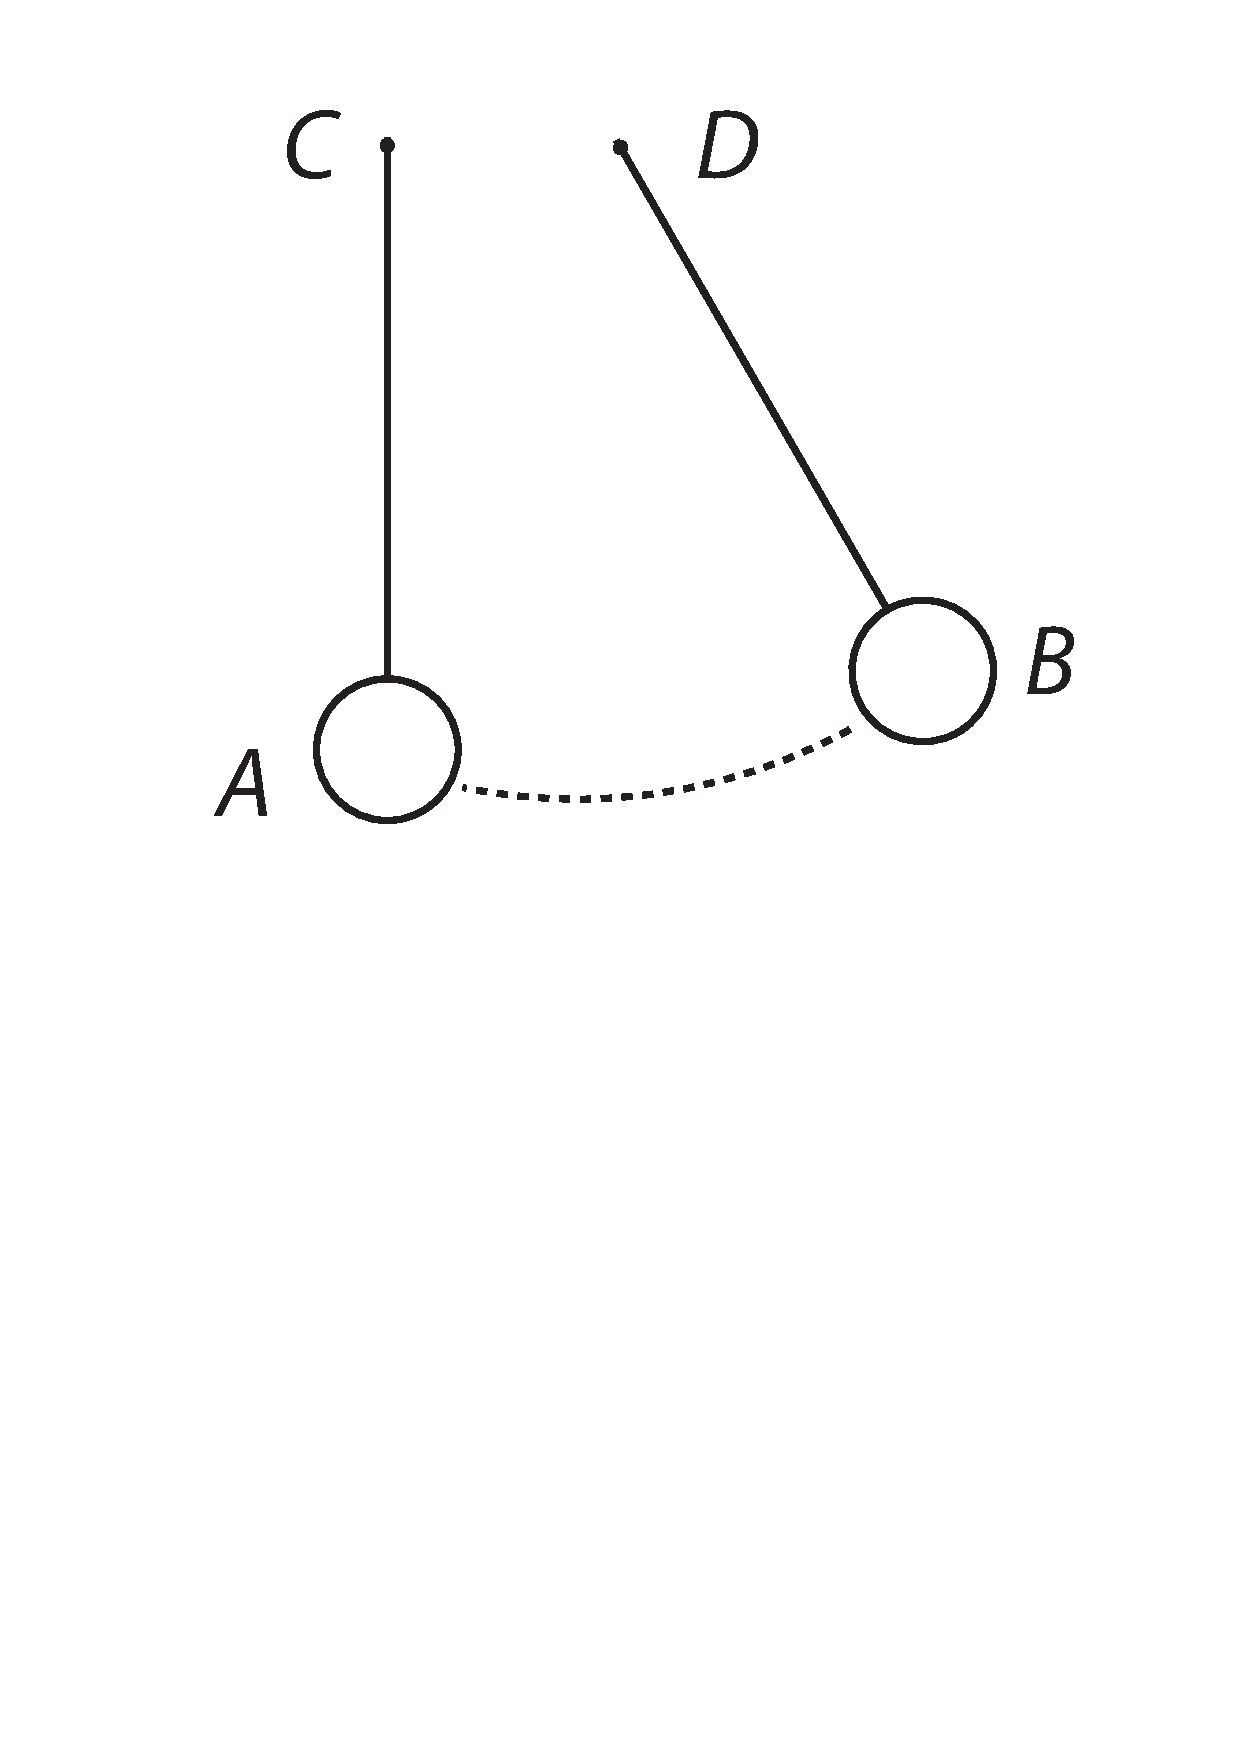
\includegraphics[trim = 0mm 0mm 0mm 0mm, clip, width=0.5\textwidth] {images/lh0351303_035r-d1.pdf}
\end{minipage}
%\hspace*{13,3mm}
\begin{minipage}[c]{0.5\textwidth}
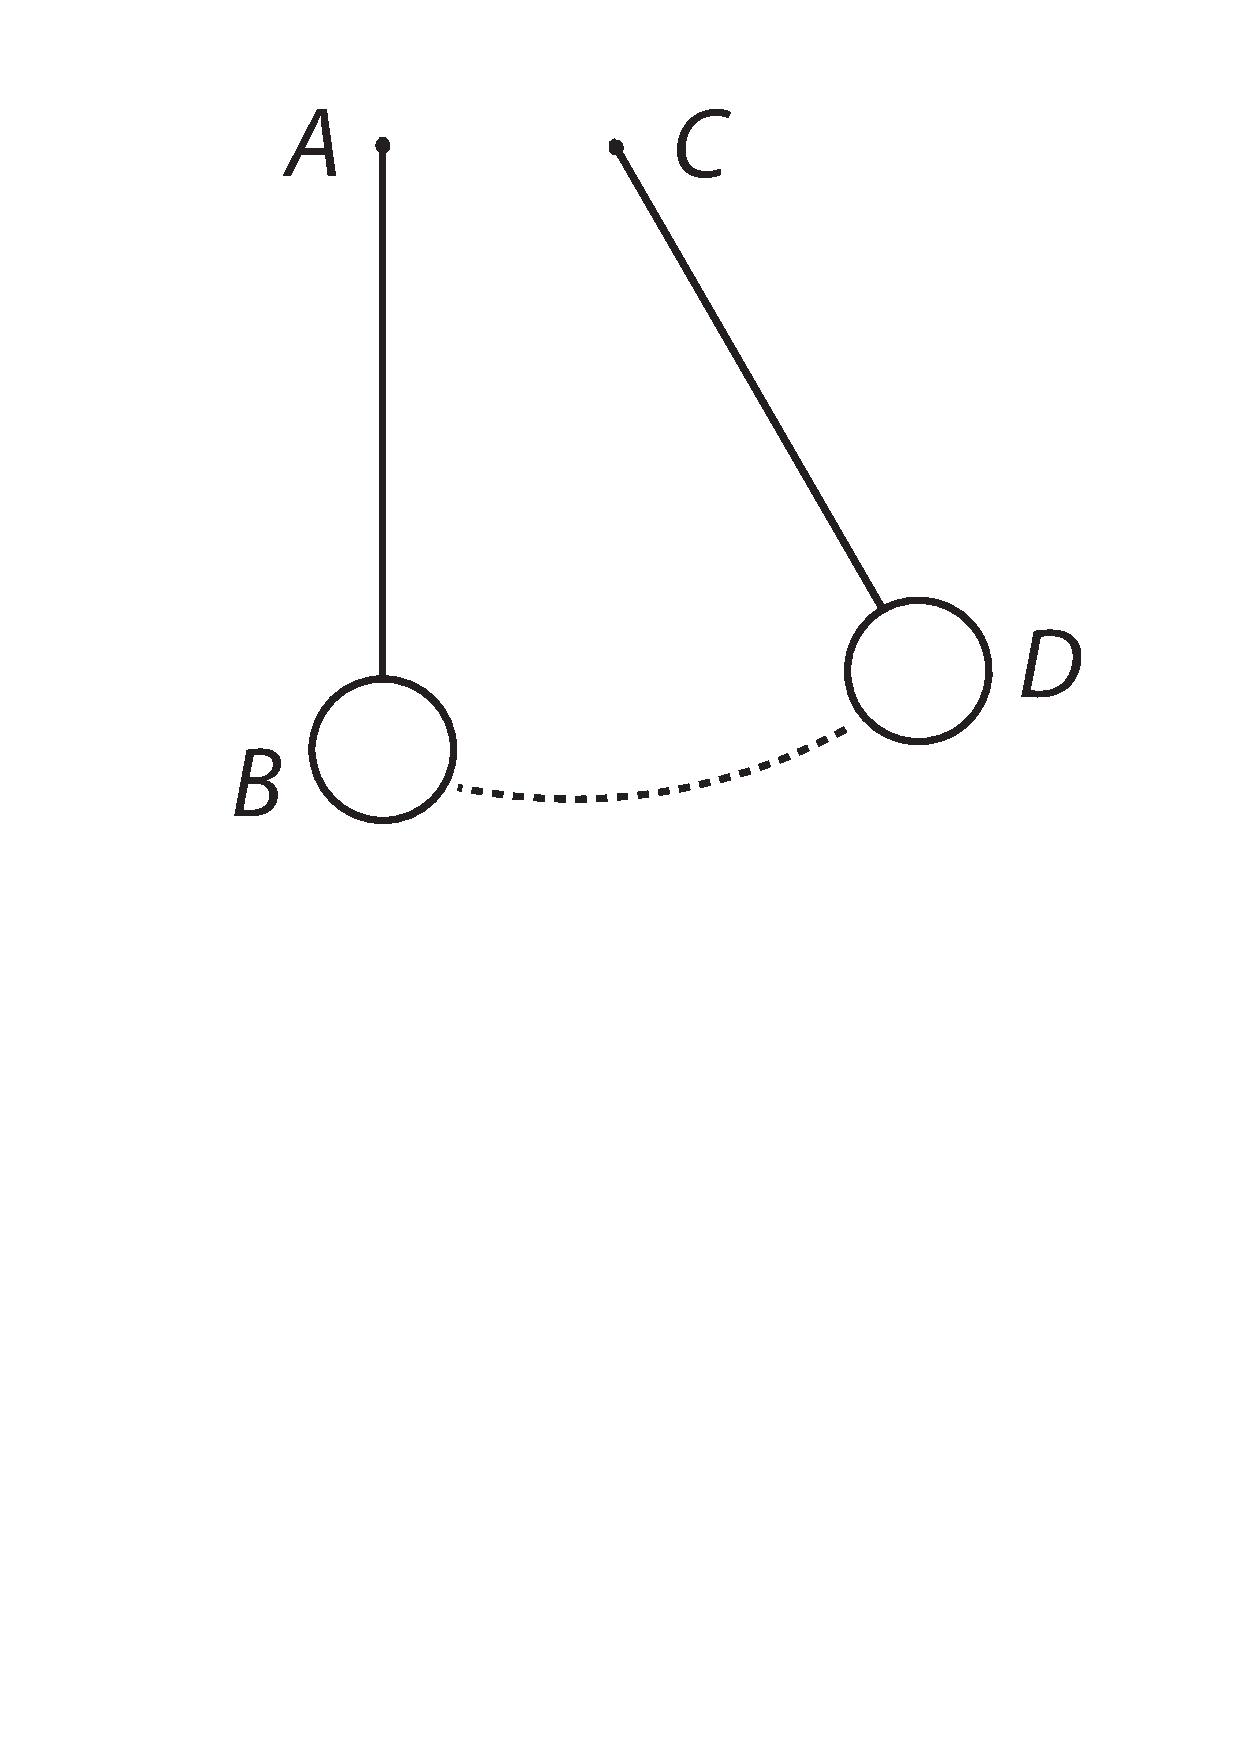
\includegraphics[trim = 0mm 0mm 0mm 0mm, clip, width=0.5\textwidth] {images/lh0351303_035r-d2.pdf}
\end{minipage}
\pend
\pstart
\vspace{1em}
\hspace*{14mm} [\textit{Fig. 1, gestr.}]\hspace*{50mm} [\textit{Fig. 2}]
%\vspace*{1em}
\pend
\newpage
\pstart
\rule[-4mm]{0mm}{10mm}%
Pone \( \displaystyle AB \, \sqcap \, x \, \sqcap \, GW \, \edtext{\sqcap \, z \).
\( \displaystyle WL \, \sqcap \, \dfrac{ a \beta }{ x }. \) }{ \lemma{$\sqcap \  z.$} \Bfootnote{\textit{(1)} $  \displaystyle WL \, \sqcap \, \dfrac{ a z }{ x } $ \textit{(2)} $ \displaystyle WL \, \sqcap \, \dfrac{ z } { x } $ \textit{(3)} $ \displaystyle WL \, \sqcap \, \dfrac{ a \beta }{ x } $ \textit{L}}}
Sed si \edtext{pro \textit{z},}{\lemma{pro} \Bfootnote{\textit{(1)}\ $\beta$ \textit{(2)}\ \textit{z} \textit{L}}}
ponamus \( \displaystyle \dfrac{y}{a} \, \beta \), erit \( \displaystyle x  \, \sqcap \, \dfrac{y^{2}}{2a}\),
et \edtext{ \( \displaystyle  WL \, \sqcap \, \dfrac{ \uline{\, a\beta \,}} { \dfrac{y^{2}}{2a} } \, \sqcap \dfrac{2a^{2} \beta}{y^{2}}. \) }{\lemma{et} \Bfootnote{\textit{(1)} $  \displaystyle WL \, \sqcap \, \dfrac{ \dfrac{a\beta}{a}} { \dfrac{y^{2}}{2a}} $ \textit{(2)} $ \displaystyle WL \, \sqcap \, {\dfrac{ 2a\beta } { }} $  \textit{(3)}  $ \displaystyle WL \, \sqcap \, \dfrac{ \uline{\, a\beta \,}} { \dfrac{y^{2}}{2a} } \, \sqcap \dfrac{2^{2} \beta}{y^{2}}$ \textit{L}}}
\pend
\count\Bfootins=1200
\count\Afootins=1200
\count\Cfootins=1200
\pstart
\vspace*{0.5em}
Ergo curva \textit{AGL} quadratrix\protect\index{Sachverzeichnis}{quadratrix}
\edtext{Hyperbolae\protect\index{Sachverzeichnis}{hyperbola} intelligi potest, descripta duobus motibus compositis, vel ex}%
{\lemma{Hyperbolae}\Bfootnote{%
\textit{(1)}\ composita %
\textit{(2)}\ intelligi potest, %
\textit{(a)} ex %
\textit{(b)} descripta [...] vel ex \textit{L}}}
uniformi, et uniformiter crescentium reciproco, vel uniformiter crescente, et uniformiter crescentium quadratis reciproco.
\pend
\vspace{1.5em}
\pstart
\noindent
\centering
%%\begin{wrapfigure}[9]{l}{0.22\textwidth}
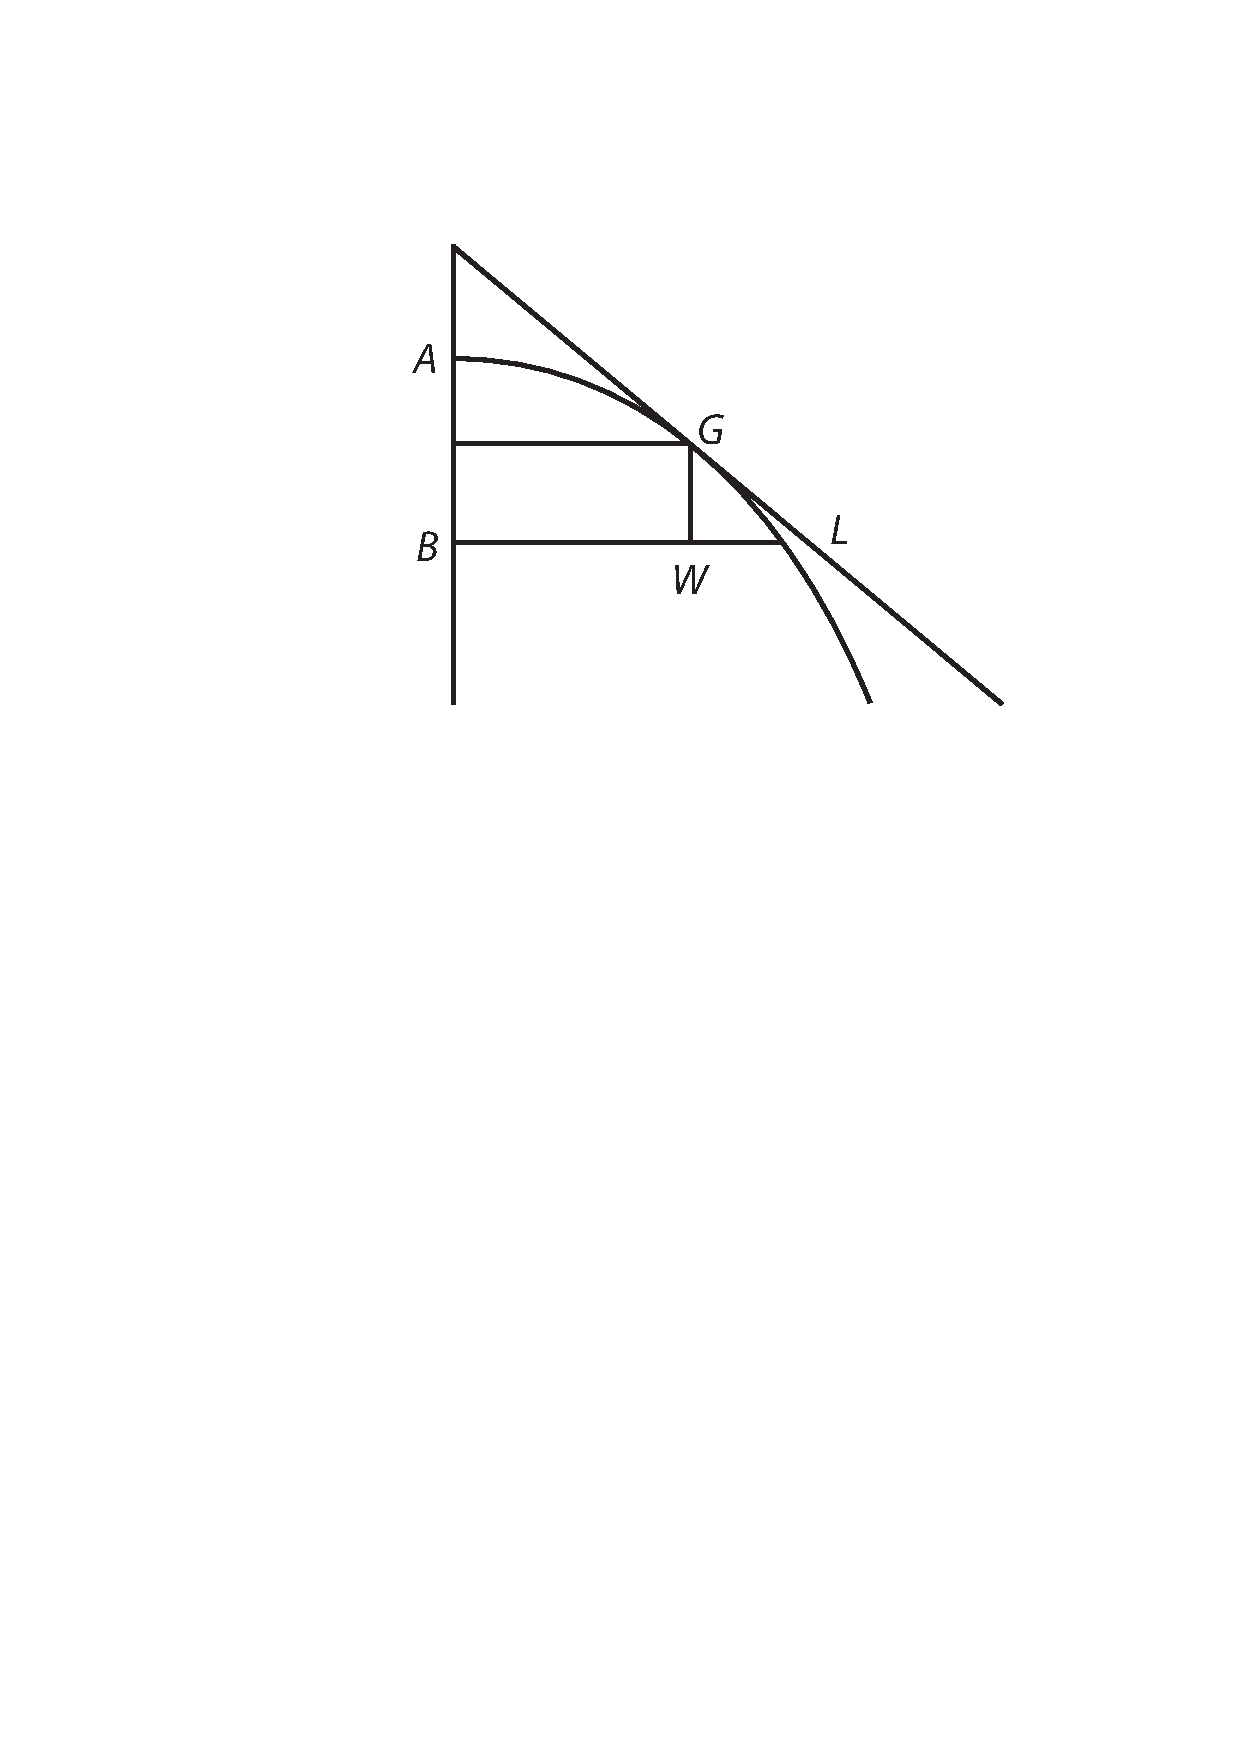
\includegraphics[trim = 0mm 0mm 0mm 0mm, clip, width=0.36\textwidth]{images/lh0351303_035r-d3.pdf}\\
\centering [\textit{Fig. 3}]
%\end{wrapfigure}
\pend
\pstart
%% HIER BEGINNT DIE MARGINALIE
\edtext{}{\lemma{\hspace{1.8mm}6\hspace{1.8mm}}\killnumber\Afootnote{\textit{Am Rand und um die Zeichnung Fig. 3:}
$\sqrt{1-y^{4}}.$
Methodus generalis quadrandi figuram curvilineam quamlibet.
Dato valore ipsius \textit{WL} per datam $AB \, \sqcap \, x.$
pro \textit{x}, substituatur alius valor; ut \textit{WL}.
Substituto eo valore fiat quadrabilis tunc compositione duorum motuum,
uno in ipsius \textit{x} valore seu curvae ad quem est valor ille ordinatis, altero in ordinatis quadratricis ipsarum \textit{WL} factitiarum.
Uno transverso, altero recto, habebitur descriptio quadratricis, valoris ipsarum \textit{WL} initio datarum.
Unde facile est eligere Constructiones simplicissimas, et infinitos eandem figuram describendi modos.\vspace{-8mm}}}
%% HIER ENDET DIE MARGINALIE
\pend
\newpage
\pstart
Sed si pro \rule[-4mm]{0mm}{10mm}\textit{z} ponatur \( \displaystyle \dfrac{y^{2}\beta}{a^{2}}  \), fiet \( \displaystyle x \, \sqcap \, \dfrac{y^{3}}{3a^{2}}  \) et \( \displaystyle WL \, \sqcap \, \dfrac{3a^{3}\beta}{y\beta}\).\rule[-4mm]{0mm}{10mm} Quanta sit vis percussionis\protect\index{Sachverzeichnis}{vis percussionis} a nemine satis explicatum arbitror. Pone \edtext{grave dati ponderis\protect\index{Sachverzeichnis}{pondus} ex data altitudine super}%
{\lemma{grave}\Bfootnote{%
\textit{(1)}\ in %
\textit{(a)}\ alteram %
\textit{(b)}\ lanc %
\textit{(c)}\ mo %
\textit{(2)}\ dati ponderis %
\textbar\ ex data altitudine \textit{erg.} \textbar\ super \textit{L}}}
lancem\protect\index{Sachverzeichnis}{lanx} librae\protect\index{Sachverzeichnis}{libra} cadere, quaeritur, quoties suum pondus in altera librae lance elevare possit. Est haec quaestio inter mechanicarum maximas habenda. Hactenus enim vires mortuas\protect\index{Sachverzeichnis}{vis mortua}, seu pondera, aut etiam vires vivas\protect\index{Sachverzeichnis}{vis viva} seu ictus\protect\index{Sachverzeichnis}{ictus} inter se comparavere Geometrae, sed nunc primum vires mortuae\protect\index{Sachverzeichnis}{vis mortua} vivis\protect\index{Sachverzeichnis}{vis viva} credo comparan\-tur. \edtext{Vim autem}{\lemma{comparantur.}\Bfootnote{\textit{(1)}\ Sane \textit{(2)}\ Vim autem \textit{L}}} mortuam\protect\index{Sachverzeichnis}{vis mortua} voco, ponderis quieti, qua ele\-va\-tioni suae aut loco motioni resistit; vivam\protect\index{Sachverzeichnis}{vis viva} vero, quam acceleratione successiva quaesivit. R. P. 
%\begin{wrapfigure}[9]{l}{0.38\textwidth}
%\vspace{-4mm}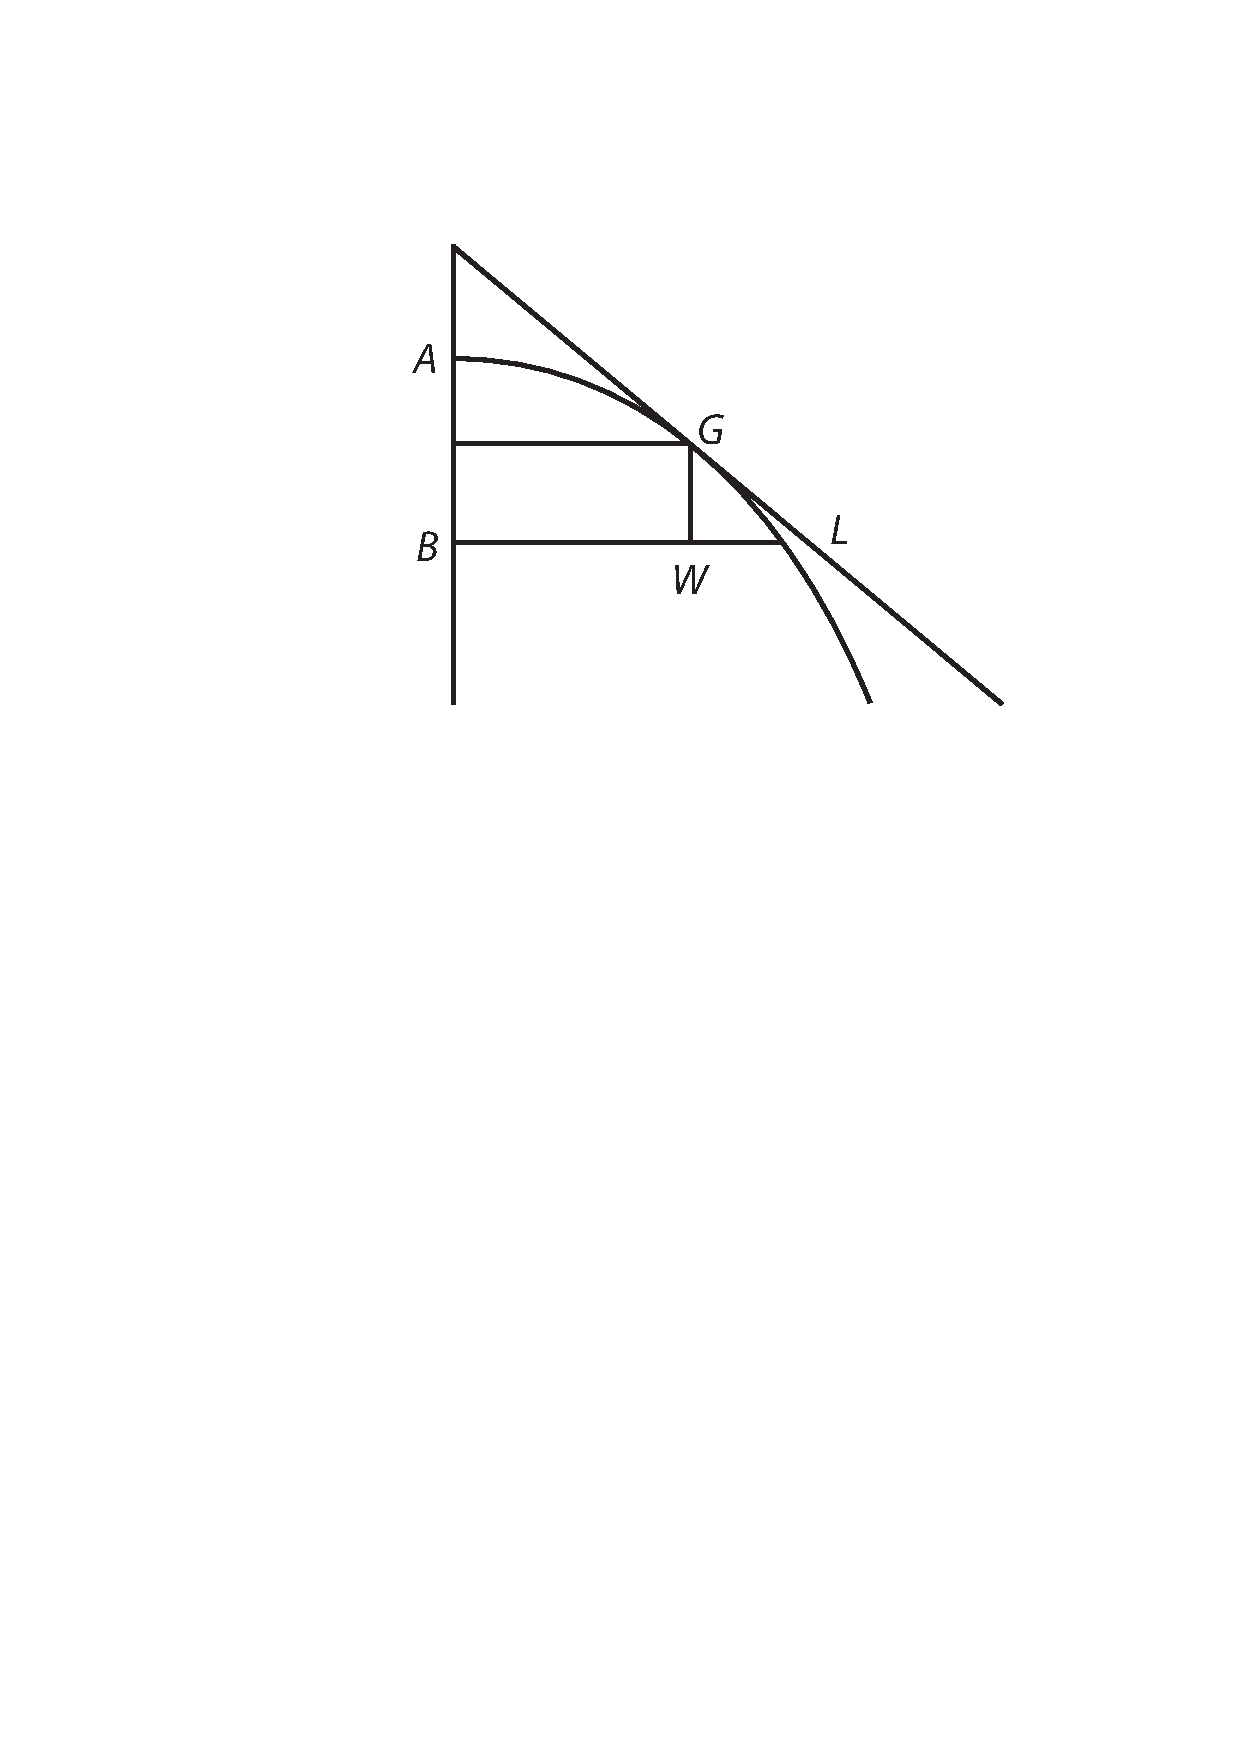
\includegraphics[width=0.38\textwidth]{images/lh0351303_035r-d3.pdf}\\
%\rule[0cm]{13mm}{0cm}[\textit{Fig. 3}]
%\end{wrapfigure}
%\edtext{}{\Afootnote{\textit{Am Rand und um die Zeichnung Fig. 3:} $ \sqrt{1-y^{4}} $ Methodus generalis quadrandi figuram curvilineam quamlibet. Dato valore ipsius \textit{WL} per datam $ AB \, \sqcap \, x $ pro \textit{x}, substituatur alius valor; ut tunc \textit{WL} substituto eo valore fiat quadrabilis tunc compositione duorum motuum, uno in ipsius \textit{x} valore seu curvae ad quem est valor ille ordinatis, altero in ordinatas quadratricis ipsarum \textit{WL} \edtext{factitiarum.}{\lemma{}\Bfootnote{factitiarum \textit{erg.} \textit{L}} uno transverso, altero recto habebitur descriptio quadratricis, valoris ipsarum \textit{WL} initio datarum unde facile est eligere constructiones simplicissimas, et infinitos eandem figuram describendi modos.}\vspace{-4mm}}} Sed si pro \rule[-4mm]{0mm}{10mm}\textit{z} ponatur \( \displaystyle \dfrac{y^{2}\beta}{a^{2}}  \), fiet \( \displaystyle x \, \sqcap \, \dfrac{y^{3}}{3a^{2}}  \) et \( \displaystyle WL \, \sqcap \, \dfrac{3a^{3}\beta}{y\beta}\).\rule[-4mm]{0mm}{10mm} Quanta sit vis percussionis\protect\index{Sachverzeichnis}{vis percussionis} a nemine satis explicatum arbitror. Pone grave \edtext{dati ponderis\protect\index{Sachverzeichnis}{pondus} ex data altitudine super lancem\protect\index{Sachverzeichnis}{lanx}}{\lemma{8f. \hspace{1.8mm} grave}\killnumber\Bfootnote{\textit{(1)} in \textit{(a)} alteram \textit{(b)} lanc \textit{(c) }mo\ \textit{(2) }dati ponderis  \textbar ex data altitudine \textit{erg.}\textbar\ super lancem \ \textit{L}}} librae\protect\index{Sachverzeichnis}{libra} cadere, quaeritur, quoties suum pondus in altera librae lance elevare possit. Est haec quaestio inter mechanicarum maximas habenda. Hactenus enim vires mortuas\protect\index{Sachverzeichnis}{vis mortua}, seu pondera, aut etiam vires vivas\protect\index{Sachverzeichnis}{vis viva} seu ictus\protect\index{Sachverzeichnis}{ictus} inter se comparavere Geometrae, sed nunc primum vires mortuae\protect\index{Sachverzeichnis}{vis mortua}
Kircherus\protect\index{Namensregister}{\textso{Kircher}, Athanasius (1601-1680) SJ} \edtext{alicubi}{\lemma{alicubi}\Cfootnote{Stelle nicht nachgewiesen.}} meminit se expertum, 20 et ultra pilas, ab una ex mediocri distantia labente elevatas. Alii sibi persuasere inde duci posse perennem \edtext{motum;\protect\index{Sachverzeichnis}{motus perennis}
Galilaeus\protect\index{Namensregister}{\textso{Galilei} (Galilaeus, Galileus), Galileo 1564-1642}}%
{\lemma{motum;}\Bfootnote{\textit{(1)}\ vir quidam doctissimus conj \textit{(2)}\ Galilaeus \textit{L}}}%
\edtext{}{\lemma{Galilaeus}\Cfootnote{%
Vermutlich Anspielung auf Galileis Abhandlung \textit{Le mecaniche} in der französischen Übersetzung von Marin Mersenne.
Siehe \cite{01091}G. \textsc{Galilei}, \textit{Les mechaniques}, Paris 1634,  S.~69-73.}}
et post eum
\edtext{Borellus,\protect\index{Namensregister}{\textso{Borelli} (Borellus), Giovanni Alfonso 1608-1679}}%
{\lemma{Borellus}\Cfootnote{%
\textsc{G.A. Borelli},\cite{01001} \title{De vi percussionis}, Bologna 1667, S.~192-210.}} 
cum dixissent ictum\protect\index{Sachverzeichnis}{ictus} esse infinitum, non
\edtext{ultra explicuere,}{\lemma{ultra}\Bfootnote{%
\textbar\ tamen \textit{gestr.} \textbar\ explicuere, \textit{L}}}
quasi proinde ulla inter vim mortuam\protect\index{Sachverzeichnis}{vis mortua} 
et vivam comparatio cessaret, velut inter finitum et infinitum.
\edtext{Vir quidam}{\lemma{Vir quidam}\Cfootnote{%
\textsc{E. Mariotte}, \cite{00311}\title{Trait\'{e} de la percussion}, Paris 1673, S.~257f.}}
nostris temporibus,\protect\index{Namensregister}{\textso{Mariotte}, Edme, Seigneur de Chazeuil ca. 1620-1684}
in experimentis\protect\index{Sachverzeichnis}{experimentum} inveniendis et explicandis
\edtext{ingeniosissimus, sentit}{\lemma{ingeniosissimus} \Bfootnote{\textit{(1)}\ credit \textit{(2)}\ sentit \textit{L}}}
guttam\protect\index{Sachverzeichnis}{gutta} aquae lapsu\protect\index{Sachverzeichnis}{lapsus} suo
\edtext{praecise cylindrum}{\lemma{praecise}\Bfootnote{\textit{(1)}\ guttam \textit{(2)}\ cylindrum \textit{L}}}
aquae sustinere ejus altitudinis, unde lapsa est, et ejusdem cum gutta\protect\index{Sachverzeichnis}{gutta} basis,
unde negat vim ictus\protect\index{Sachverzeichnis}{ictus} esse infinitam, aut certe tam magnam quam faciunt.
\newline%
\indent%
Ego in hoc negotio investigando ita processi.
\pend
\vspace{1.5em}
\pstart
\noindent
\centering
%%\begin{wrapfigure}[9]{l}{0.22\textwidth}
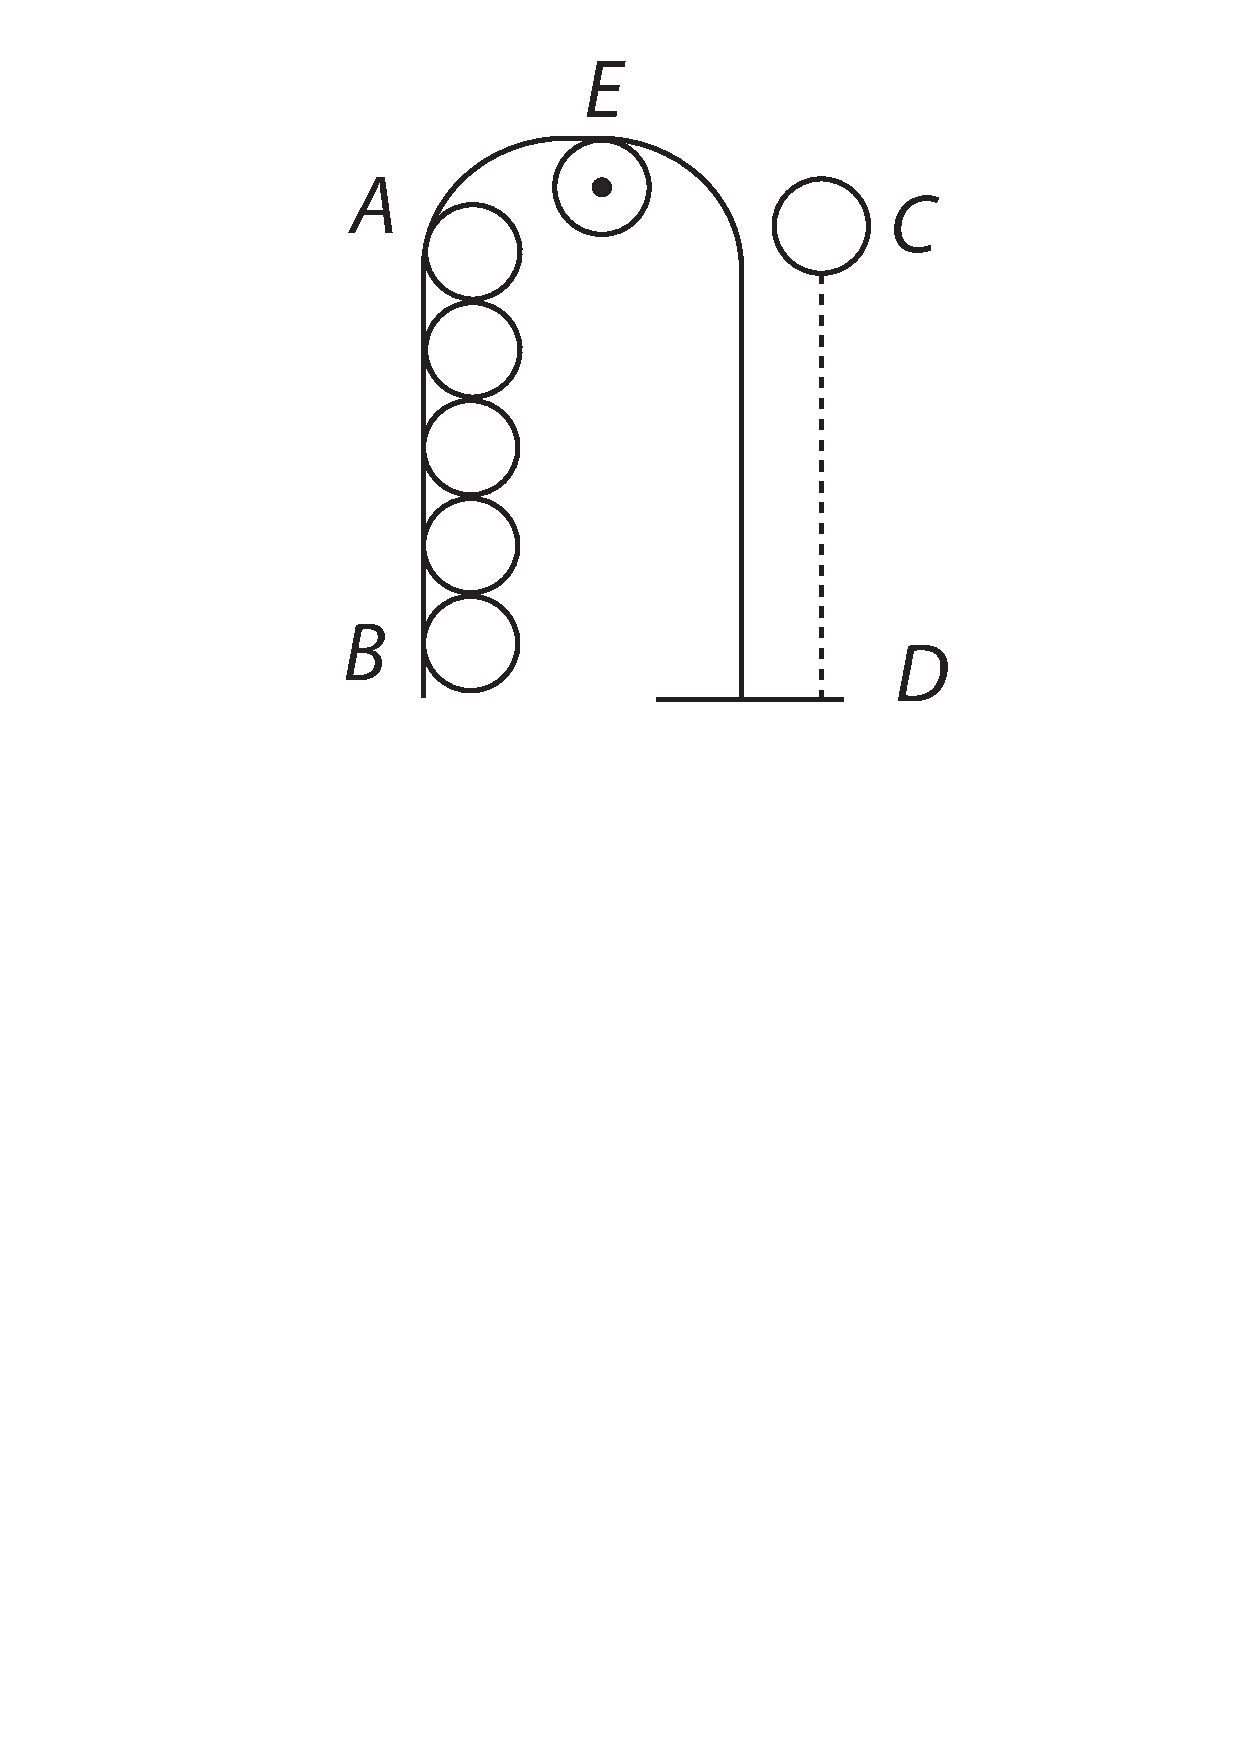
\includegraphics[trim = 0mm 0mm 0mm 0mm, clip, width=0.23\textwidth]{images/lh0351303_035r-d4.pdf}\\
\centering [\textit{Fig. 4}]
%\end{wrapfigure}
\pend
\count\Bfootins=1200
\count\Afootins=1200
\count\Cfootins=1200
\vspace{1.5em}
\pstart  
%\begin{wrapfigure}[9]{l}{0.22\textwidth}
%\vspace{-3mm}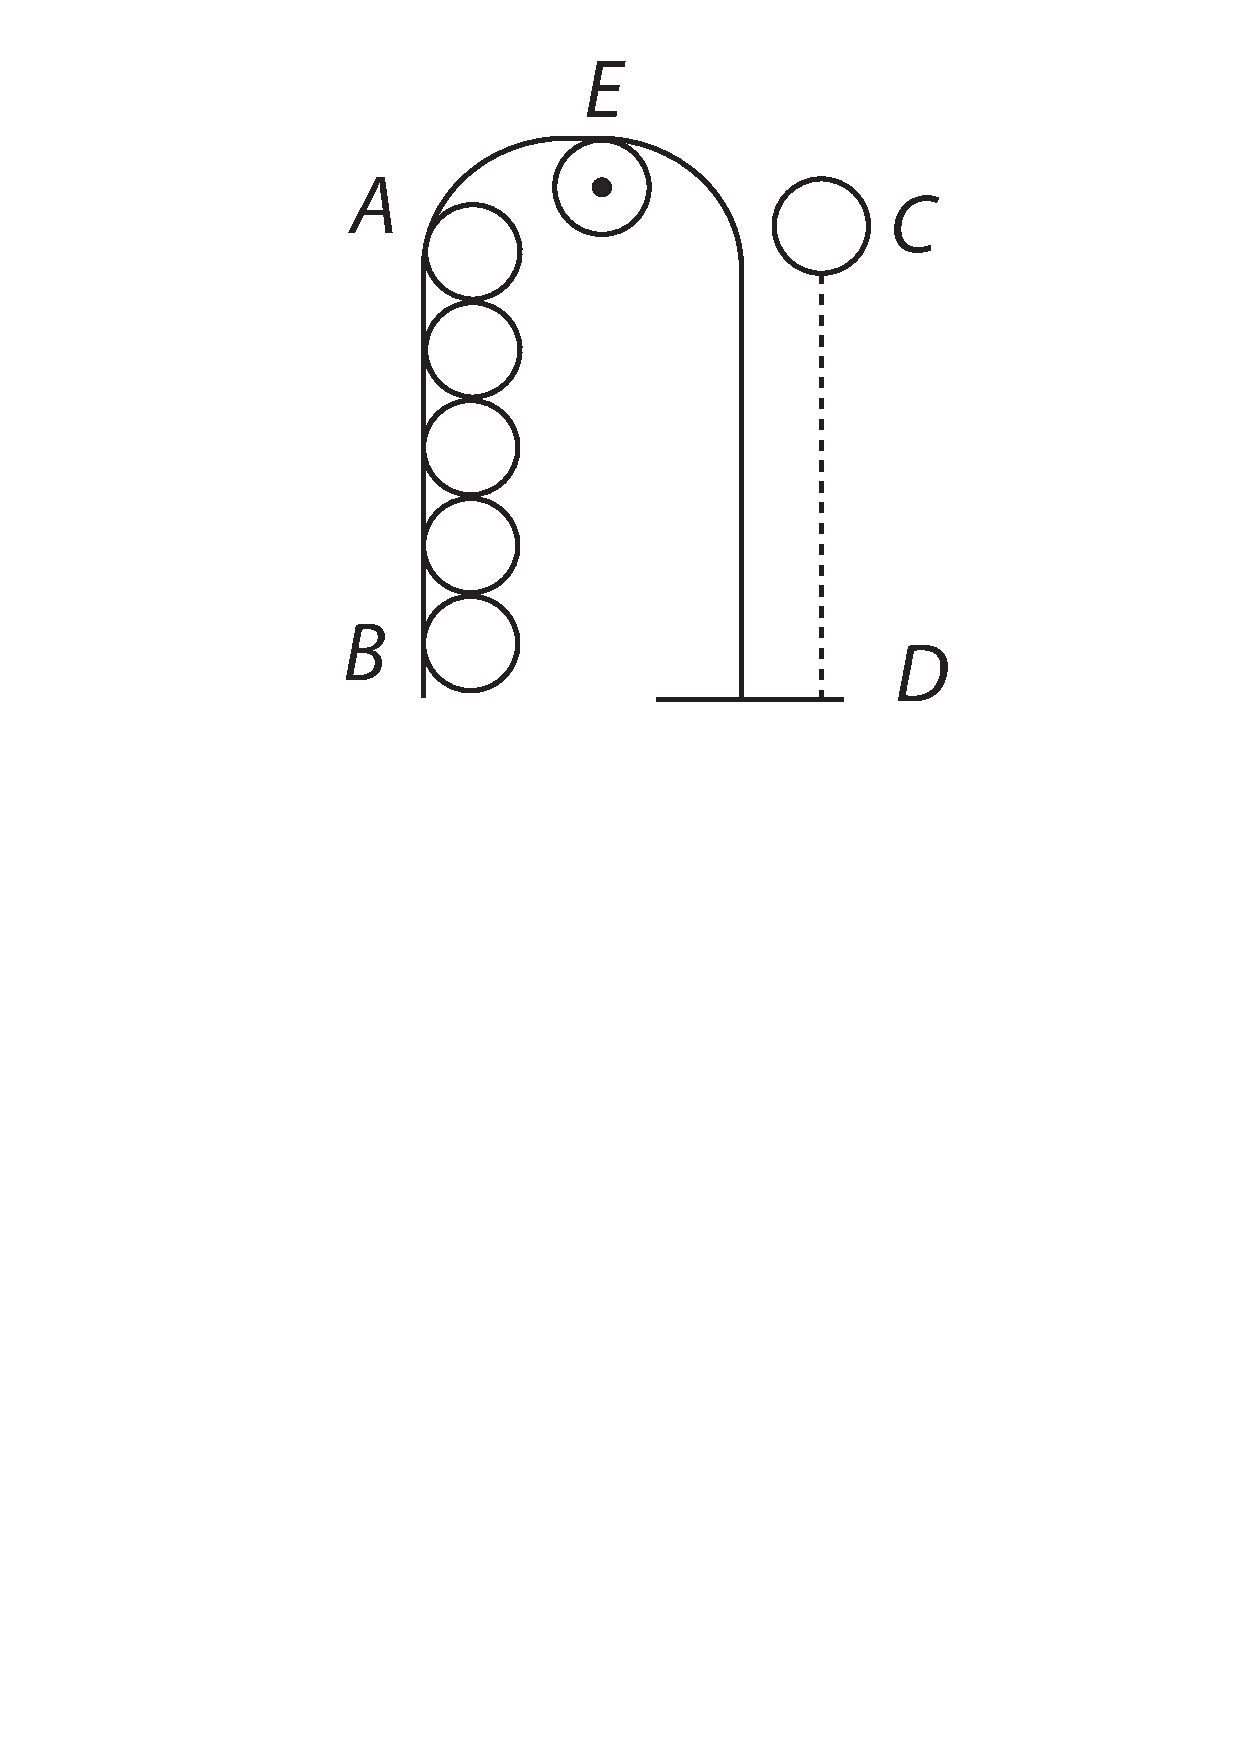
\includegraphics[trim = 0mm -2mm -5mm 0mm, clip, width=0.22\textwidth]{images/lh0351303_035r-d4.pdf}\\
%\centering [\textit{Fig. 4}]
%\end{wrapfigure}
\noindent
Fingatur catena \edtext{globorum contiguorum}{\lemma{catena} \Bfootnote{\textit{(1)}\ corporum ita \textit{(2)}\ globorum contiguorum \textit{L}\ }} \textit{AB} unde summa \textit{C}, cadens in patinam \textit{D}, ope chordae \textit{DE} circa trochleam \textit{E}, faciat surgere catenam, et ipsa succedat in ultimae locum, summa autem rursus cadat succedatque in locum ipsius; patet inde sequi perennem motum\protect\index{Sachverzeichnis}{motus perennis}. Quod est absurdum; patet
ergo non posse tantam esse vim ictus\protect\index{Sachverzeichnis}{ictus}, quantam sufficit ad elevandam eousque catenam, ut \edtext{continuari possit}{\lemma{ut} \Bfootnote{\textit{(1)}\ attollere possit \textit{(2)}\ continuari possit \textit{L}\ }} ictus\protect\index{Sachverzeichnis}{ictus}.
\\\indent
Nimirum illud pro certo habendum est, solo lapsu\protect\index{Sachverzeichnis}{lapsus} fieri non posse, ut corpus labens, aut aliud ei aequipollens altius attollatur, quam unde lapsum\protect\index{Sachverzeichnis}{lapsus} est. Pone enim aequipollens altius attolli posse, sequitur ipsummet altius attolli posse; nam aequipollens altius sublatum cogatur in libram incidere, qua attollat datum; fiet, ut lapsus\protect\index{Sachverzeichnis}{lapsus} solus corporis dati, causa sit ascensus in locum ipso lapsu\protect\index{Sachverzeichnis}{lapsus} altiorem.
\pend
\pstart
Principium\protect\index{Sachverzeichnis}{principium} hoc tum rationibus tum experimentis\protect\index{Sachverzeichnis}{experimentum} confirmari potest; rationibus, quod natura non videatur agere contra se ipsam, experimento\protect\index{Sachverzeichnis}{experimentum}, quod pendulum sibi permissum numquam ad altitudinem priorem reascendit; cum tamen summa sit libertas ipsi; multo minus corpus ad altiorem sibi locum ascendet \edtext{per ipsam sui lapsus\protect\index{Sachverzeichnis}{lapsus} vim}{\lemma{ascendet} \Bfootnote{\textit{(1)}\ vi lap \textit{(2)}\ per ipsam sui lapsus\protect\index{Sachverzeichnis}{lapsus} vim \textit{L}\ }} in alia corpora transditam. 
\pend
%\newpage
\pstart
Sed demonstratio hujus rei altior est, quod scilicet tam est facile attollere centum libras ad unam leucam, quam unam libram ad 100 leucas, tantundem enim effectus consecuta est rerum \edtext{natura.}{\lemma{}\Afootnote{\textit{Zwischen den Zeilen, gestrichen:} Maxima pars hominum rudibus damnata tenebris.}}
\pend
\pstart
Itaque in motibus illis universalibus infatigatis, ubi semper effectum suum quantum fieri potest, consequitur rerum natura.\\
\begin{wrapfigure}{l}{\textwidth}
\centering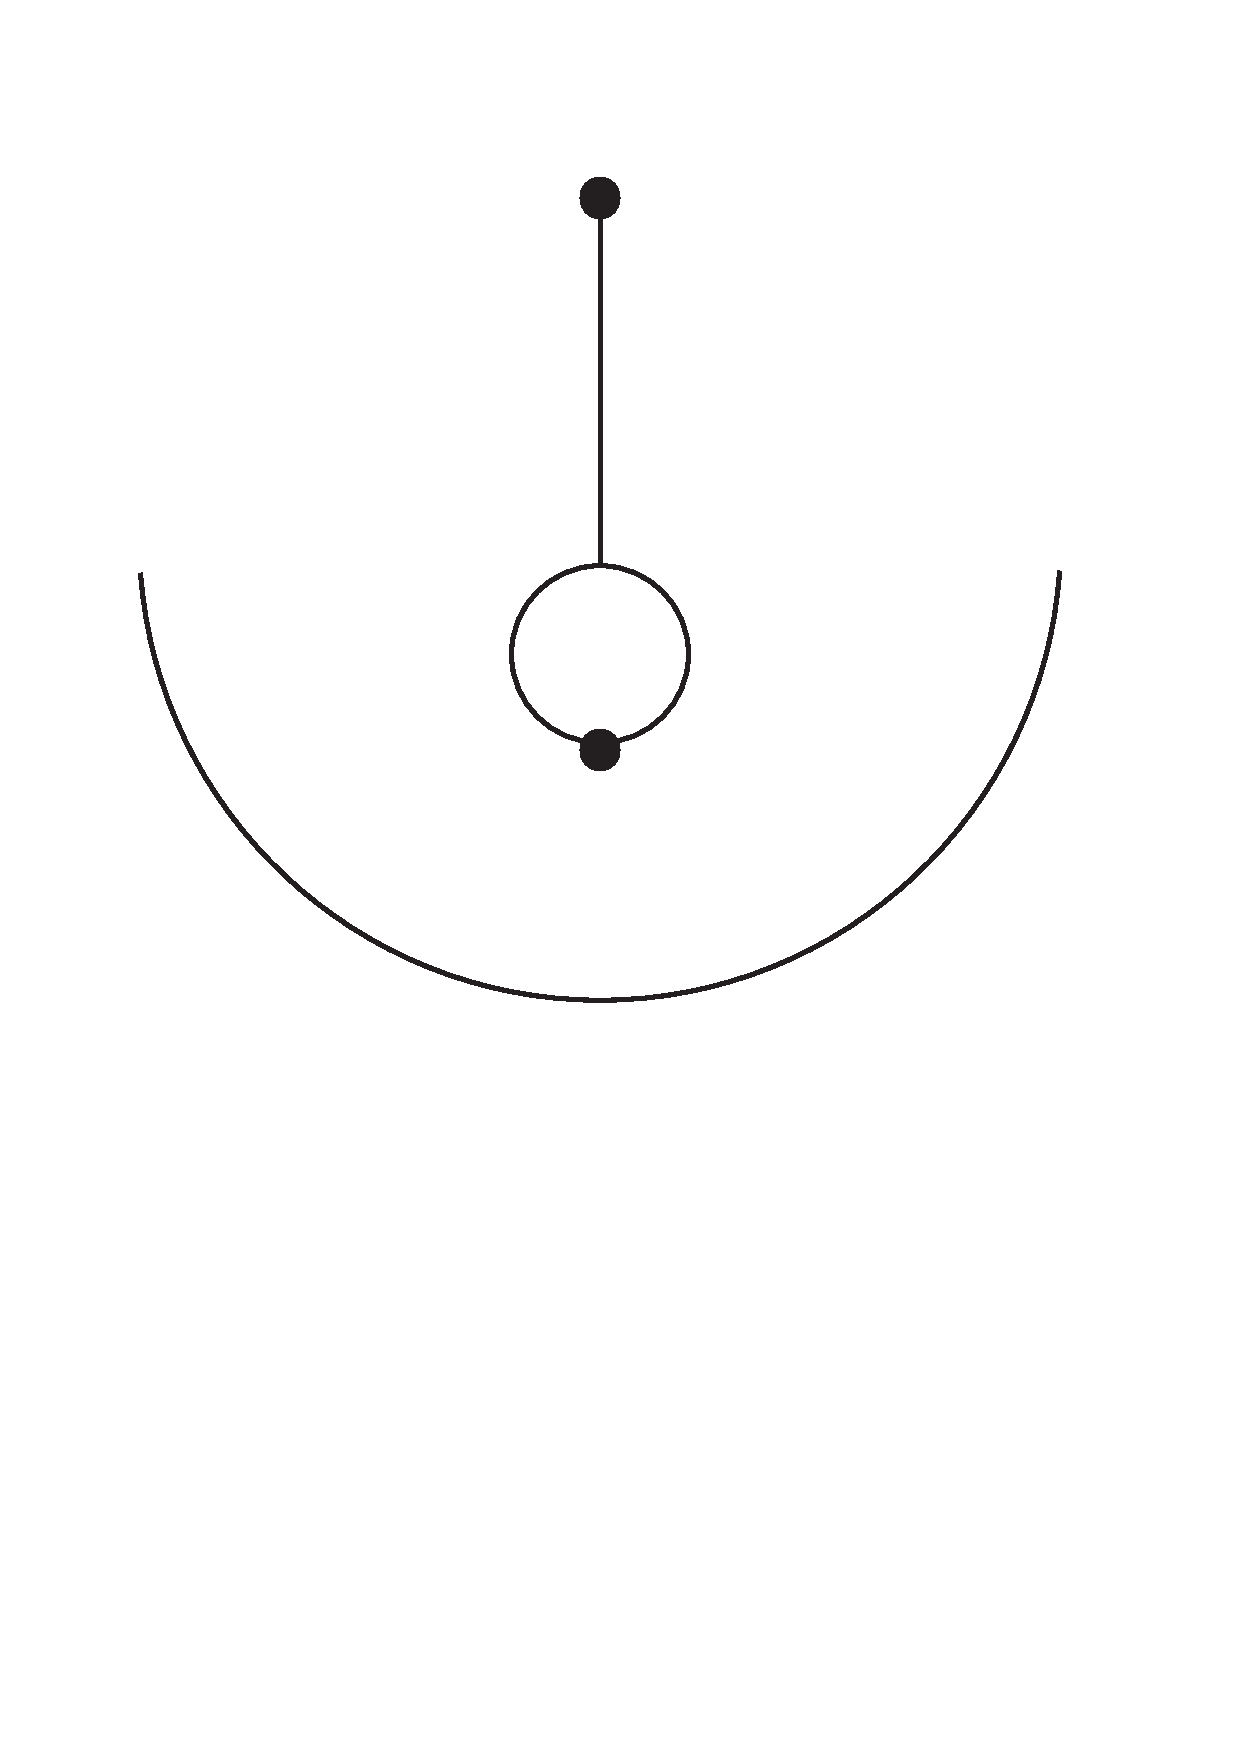
\includegraphics[width=0.2\textwidth]{images/lh0351303_035r-d5.pdf}\\
\rule[0cm]{0mm}{0cm}[\textit{Fig. 5}]
\end{wrapfigure}
\pend
\count\Afootins=1500
\count\Bfootins=1500
\count\Cfootins=1500
 

